% Options for packages loaded elsewhere
\PassOptionsToPackage{unicode}{hyperref}
\PassOptionsToPackage{hyphens}{url}
%
\documentclass[
  12pt,
]{article}
\usepackage{amsmath,amssymb}
\usepackage{lmodern}
\usepackage{setspace}
\usepackage{iftex}
\ifPDFTeX
  \usepackage[T1]{fontenc}
  \usepackage[utf8]{inputenc}
  \usepackage{textcomp} % provide euro and other symbols
\else % if luatex or xetex
  \usepackage{unicode-math}
  \defaultfontfeatures{Scale=MatchLowercase}
  \defaultfontfeatures[\rmfamily]{Ligatures=TeX,Scale=1}
\fi
% Use upquote if available, for straight quotes in verbatim environments
\IfFileExists{upquote.sty}{\usepackage{upquote}}{}
\IfFileExists{microtype.sty}{% use microtype if available
  \usepackage[]{microtype}
  \UseMicrotypeSet[protrusion]{basicmath} % disable protrusion for tt fonts
}{}
\usepackage{xcolor}
\usepackage[margin=1in]{geometry}
\usepackage{longtable,booktabs,array}
\usepackage{calc} % for calculating minipage widths
% Correct order of tables after \paragraph or \subparagraph
\usepackage{etoolbox}
\makeatletter
\patchcmd\longtable{\par}{\if@noskipsec\mbox{}\fi\par}{}{}
\makeatother
% Allow footnotes in longtable head/foot
\IfFileExists{footnotehyper.sty}{\usepackage{footnotehyper}}{\usepackage{footnote}}
\makesavenoteenv{longtable}
\usepackage{graphicx}
\makeatletter
\def\maxwidth{\ifdim\Gin@nat@width>\linewidth\linewidth\else\Gin@nat@width\fi}
\def\maxheight{\ifdim\Gin@nat@height>\textheight\textheight\else\Gin@nat@height\fi}
\makeatother
% Scale images if necessary, so that they will not overflow the page
% margins by default, and it is still possible to overwrite the defaults
% using explicit options in \includegraphics[width, height, ...]{}
\setkeys{Gin}{width=\maxwidth,height=\maxheight,keepaspectratio}
% Set default figure placement to htbp
\makeatletter
\def\fps@figure{htbp}
\makeatother
\setlength{\emergencystretch}{3em} % prevent overfull lines
\providecommand{\tightlist}{%
  \setlength{\itemsep}{0pt}\setlength{\parskip}{0pt}}
\setcounter{secnumdepth}{-\maxdimen} % remove section numbering
\newlength{\cslhangindent}
\setlength{\cslhangindent}{1.5em}
\newlength{\csllabelwidth}
\setlength{\csllabelwidth}{3em}
\newlength{\cslentryspacingunit} % times entry-spacing
\setlength{\cslentryspacingunit}{\parskip}
\newenvironment{CSLReferences}[2] % #1 hanging-ident, #2 entry spacing
 {% don't indent paragraphs
  \setlength{\parindent}{0pt}
  % turn on hanging indent if param 1 is 1
  \ifodd #1
  \let\oldpar\par
  \def\par{\hangindent=\cslhangindent\oldpar}
  \fi
  % set entry spacing
  \setlength{\parskip}{#2\cslentryspacingunit}
 }%
 {}
\usepackage{calc}
\newcommand{\CSLBlock}[1]{#1\hfill\break}
\newcommand{\CSLLeftMargin}[1]{\parbox[t]{\csllabelwidth}{#1}}
\newcommand{\CSLRightInline}[1]{\parbox[t]{\linewidth - \csllabelwidth}{#1}\break}
\newcommand{\CSLIndent}[1]{\hspace{\cslhangindent}#1}
\usepackage{setspace}\doublespacing
\usepackage{fontspec}
\setmainfont{Times New Roman}
\usepackage{placeins}
\usepackage{lineno}
\usepackage{amsmath}
\numberwithin{equation}
\usepackage{indentfirst}
\linenumbers
\ifLuaTeX
  \usepackage{selnolig}  % disable illegal ligatures
\fi
\IfFileExists{bookmark.sty}{\usepackage{bookmark}}{\usepackage{hyperref}}
\IfFileExists{xurl.sty}{\usepackage{xurl}}{} % add URL line breaks if available
\urlstyle{same} % disable monospaced font for URLs
\hypersetup{
  pdftitle={A Bayesian hierarchical model for size spectra},
  hidelinks,
  pdfcreator={LaTeX via pandoc}}

\title{A Bayesian hierarchical model for size spectra}
\author{true \and true \and true \and true \and true}
\date{}

\begin{document}
\maketitle

\setstretch{1}
\newpage

\hypertarget{abstract}{%
\section{Abstract}\label{abstract}}

A fundamental pattern in ecology is that smaller organisms are more
abundant than larger organisms. This pattern is described by the
individual size distribution (ISD), which is the frequency of all
individual sizes in an ecosystem, regardless of taxon. The ISD is
described by power law distribution with the form
\(f(x) = cx^{\lambda}\), and a major goal of size spectra analyses is to
estimate the ISD parameter \(\lambda\). However, while numerous methods
have been developed to do this, they have focused almost exclusively on
estimating \(\lambda\) from single samples. Here, we develop an
extension of the truncated Pareto distribution within the probabilistic
modeling language Stan. We use it to estimate multiple ISD parameters
simultaneously with a hierarchical modeling approach. The most important
result is the ability to examine hypotheses related to size spectra,
including the assessment of fixed and random effects, within a single
Bayesian generalized (non)-linear mixed model.

Keywords: \emph{Bayesian, body size spectra, hierarchical, Pareto, power
law, Stan}

\newpage

\hypertarget{introduction}{%
\section{Introduction}\label{introduction}}

In any ecosystem, large individuals are typically more rare than small
individuals. This fundamental feature of ecosystems leads to a
remarkably common pattern in which relative abundance declines with
individual body size, generating the individual size distribution ISD
(or community size spectrum) (Sprules et al. 1983, White et al. 2008).
Understanding how body sizes are distributed has been a focus in ecology
for over a century (Peters and Wassenberg 1983), in part because they
represent an ataxic approach that reflects fundamental measures of
ecosystem structure and function, such as trophic transfer efficiency.
(Kerr and Dickie 2001, White et al. 2007, Perkins et al. 2019).
Individual size distributions are also predicted as a result of
physiological limits associated with body size, thereby emerging from
predictions of metabolic theory and energetic equivalence (Brown et al.
2004).

More formally, the ISD is a frequency distribution that can be
approximated by a bounded power law with a single free parameter
\(\lambda\), corresponding to the following probability density function
(Edwards et al. 2020):

\[
f(x) = Cx^\lambda, x_{min} \le x \ge x_{max}
\]

where \(x\) is the body size (e.g., mass or volume) of an individual
regardless of taxon, \(x_{min}\) is the smallest individual attainable
and \(x_{max}\) is the largest possible individual (White et al. 2008).
\(C\) is a constant equal to:

\[
 C = \begin{cases}\frac{\lambda + 1}{{x_{max}^{\lambda+1}} - {x_{min}^{\lambda+1}}}, \lambda \neq-1 \\
\frac{1}{{logx_{max}} - {logx_{min}}}, \lambda = -1\end{cases}
\]

This model is also known as the bounded power law or truncated Pareto
distribution. The terms ``bounded'' or ``truncated'' refer to the limits
of \(x_{min}\) and \(x_{max}\), which represent the minimum and maximum
attainable body size values (White et al. 2008). In practice, values of
\(x_{min}\) and \(x_{max}\) often come from the minimum and maximum body
sizes in a data set or are estimated statistically (White et al. 2008,
Edwards et al. 2017).

A compelling feature of size spectra is that \(\lambda\) may vary little
across ecosystems as a result of physiological constraints that lead to
size-abundance patterns more broadly. Metabolic scaling theory predicts
\(\lambda + 1 = \frac{log\alpha}{log\beta} - 3/4\), where \(\alpha\) is
trophic transfer efficiency in the food web and \(\beta\) is the mean
predator-prey mass ratio in a community (Reuman et al. 2008). The value
of \(-3/4\) is the predicted scaling exponent of log abundance and log
mass (Damuth 1981, Peters and Wassenberg 1983). It is the reciprocal of
scaling coefficient of metabolic rate and mass (0.75) (Brown et al.
2004) and as a result, values of \(\lambda + 1\) have been used to
estimate metabolic scaling across ecosystems Perkins et al. (2019).
Because \(\frac{log\alpha}{log\beta}\) is typically
\textless\textless0.01, this implies that a \(\lambda\) values of
\textasciitilde-1.75 represent a reasonable first guess of expected ISD
exponents, with values of ranging from -1.2 to -2 often appearing in the
literature (Andersen and Beyer 2006, Blanchard et al. 2009, Pomeranz et
al. 2020b).

Whether \(\lambda\) represents a fixed or variable value is debated, but
it often varies among samples and ecosystems (Blanchard et al. 2009,
Perkins et al. 2018, Pomeranz et al. 2020b). It is often described by
its ``steepness'', with more negative values (i.e., ``steeper'')
indicating lower abundance of large relative to small individuals, and
vice versa. These patterns of size frequency are an emergent property of
demographic processes (e.g., age-dependent mortality), ecological
interactions (e.g., size-structured predation, trophic transfer
efficiency), and physiological constraints (e.g., size-dependent
metabolic rates) (Muller-Landau et al. 2006, Andersen and Beyer 2006,
White et al. 2008). As a result, variation in \(\lambda\) across
ecosystems or across time can indicate fundamental shifts in community
structure or ecosystem functioning. For example, overfishing in marine
communities has been detected using size spectra in which \(\lambda\)
was steeper than expected, indicating fewer large fish than expected
(Jennings and Blanchard 2004). Shifts in \(\lambda\) have also been used
to document responses to acid mine drainage in streams (Pomeranz et al.
2019, 2020a), land use (Martínez et al. 2016), resource subsidies
(Perkins et al. 2018), and temperature (O'Gorman et al. 2017, Pomeranz
et al. 2022).

Given the ecological information it conveys, the data required to
estimate size spectra are deceptively simple; only a single column of
data are needed, in which each data point is a single measure of the
body size of an individual. As long as the body sizes are collected
systematically and without bias towards certain taxa or phenotypes,
there is no need to know any more ecological information about the data
points (e.g., taxon, trophic position, age, abundance). However, despite
the simple data requirement, the statistical models used to estimate
\(\lambda\) are diverse. Edwards et al. (2017) documented 8 different
analytical methods. Six involved binning, in which the body sizes are
grouped into size bins (e.g., 2-49 mg, 50-150mg, etc.) and then counted,
generating values for abundance within each size bin. When both axes are
log-transformed, binning allows \(\lambda\) to be estimated using simple
linear regression. Unfortunately, the binning process also removes most
of the variation in the data, collapsing information about 1000's of
individuals into just 6 or so bins. Doing so can lead to the wrong
values of \(\lambda\), sometimes drastically so (White et al. 2008,
Edwards et al. 2017, 2020).

An improved alternative to binning and linear regression is to fit the
body size data to a power law probability distribution (White et al.
2008, Edwards et al. 2017, 2020). This method uses all raw data
observations directly to estimate \(\lambda\), typically using the
maximum likelihood estimation method (Edwards et al. 2017). In addition
to estimating size spectra of single samples, ecologists have used this
method to examine how \(\lambda\) varies across environmental gradients
(Perkins et al. 2019, Pomeranz et al. 2022). However, these analyses
typically proceed in two steps. First, \(\lambda\) estimates are
obtained individually from each collection (e.g., each site or year,
etc.). Second, these estimates are used as response variables in a
linear model to examine how they relate to corresponding predictor
variables (Edwards et al. 2020). A downside to this approach is that it
treats \(\lambda\) values as independent samples, even if they come from
the same site or time. It also removes information on sample size
(number of individuals) used to derive \(\lambda\). As a result, the
approach not only separates the data generation model from the predictor
variables, but it is also unable to take advantage of partial pooling
during model fitting.

Here, we develop a Bayesian model that uses the truncated Pareto
distribution to estimate \(\lambda\) in response to both fixed and
random predictor variables. The model extends the maximum likelihood
approach developed by Edwards et al. (2020) and allows for a flexible
hierarchical structure, including partial pooling, within the modeling
language Stan (Stan Development Team 2022).

\hypertarget{methods}{%
\section{Methods}\label{methods}}

\hypertarget{translating-to-stan}{%
\subsection{Translating to Stan}\label{translating-to-stan}}

We first translated the probability density function described by
Edwards et al. (2020) into Stan by converting it to the log probability
density function (lpdf). Stan is a probabilistic modeling language that
is capable of fitting complex models, including those with custom
lpdf's. The resulting lpdf is given as

\[
 lpdf = \begin{cases}\text{log}\frac{\lambda + 1}{{x_{max}^{\lambda+1}} - {x_{min}^{\lambda+1}}} + \lambda\text{log}x, \lambda \neq-1 \\
\text{-log}({{\text{log}x_{max}} - {\text{log}x_{min}}}) -\text{log}x, \lambda = -1\end{cases}
\]

with all variables as described above. We also show the implementation
of this and other models using Stan in the Supplementary Information.

We call this the \(paretocustom\) distribution, which we can now use to
estimate \(\lambda\) of a given data set. For example, an intercept-only
model would look like this:

\[x_i \sim paretocustom(\lambda, x_{min}, x_{max})\]
\[\lambda = \alpha\] \[\alpha \sim Normal(\mu, \sigma)\]

where \(x_i\) is the \(i\)th individual body size, \(\lambda\) is the
size spectrum parameter, \(x_{min}\) and \(x_{max}\) are as defined
above, and \(\alpha\) is the intercept with a prior probability
distribution. In this case, we specified a Normal prior since
\(\lambda\) is continuous and can be positive or negative, but this can
be changed as needed.

The simple model above can be expanded to a generalized linear mixed
model by including fixed predictors (\(\boldsymbol\beta \textbf{X}\))
and/or varying intercepts (\(\alpha_{[x]}\)):

\[x_{ij} \sim paretocustom(\lambda_j, x_{min, j}, x_{max, j})\]
\[\lambda = \alpha + \boldsymbol\beta \textbf{X} + \alpha_{[j]} + \alpha_{[x]}\]
\[\alpha \sim Normal(\mu_{\alpha}, \sigma_{\alpha})\]
\[\beta \sim Normal(\mu_{\beta},\sigma_{\beta})\]
\[\alpha_{[j]} \sim Normal(0, \sigma_{[j]})\]
\[\sigma_{[j]} \sim Exponential(\phi)\]
\[\alpha_{[x]} \sim Normal(0, \sigma_{[x]})\]
\[\sigma_{[x]} \sim Exponential(\phi)\]

with one or more \(\beta\) regression parameters, represented by the
vector \(\boldsymbol\beta\), for one or more fixed predictors
\(\textbf{X}\), and one or more varying intercepts \(\alpha_x\). We
specify \(\alpha_{j}\) separately because it is needed to account for
the non-independence of body sizes. In other words, each body size
\(x_i\) is clustered within each site and so they are not independent
and identically distributed. The addition of a varying intercept for
each sample accounts for this non-independence. We demonstrate how
excluding the sample-specific varying intercept can lead to
overdispersion below. Prior distributions are given as \(Normal\) for
the parameters and varying intercept and \(Exponential\) for
\(\sigma{[x]}\), but these can also be changed as needed.

The model above assumes that each body size \(x\) represents a single
individual such that the data set might have many repeats for
individuals of the same size (e.g., \(x\) = \{0.2, 0.2, 0.2, 0.4, 0.4,
0.5, 9.8\}). However, when individual body sizes are repeated in a data
set, they are often accompanied by a count or density, such that the
data set above might instead consist of two columns with \(x\) = \{0.2,
0.4, 0.5, 9.8\} and \(counts\) = \{3, 2, 1, 1\}. To analyze this more
compact data set, Edwards et al. (2020) developed a modification of the
log probability density function to include \(counts\):

\[
 lpdf = \begin{cases}\textit{counts}(\text{log}\frac{\lambda + 1}{{x_{max}^{\lambda+1}} - {x_{min}^{\lambda+1}}} + \lambda\text{log}x), \lambda \neq-1 \\
\textit{counts}(
\text{-log}({{\text{log}x_{max}} - {\text{log}x_{min}}}) -\text{log}x, \lambda = -1\end{cases}.
\]

We refer to this as \(paretocounts\), such that the model can be fit by
using

\[x_i\sim paretocounts(\lambda, x_{min}, x_{max}, counts)\]
\[\lambda = [\text{linear or non-linear model}] \text{ and}\]
\[\text{[priors]}.\]

Aside from adding \(counts\), the model is the same as presented above.
These models (\(paretocustom\) and \(paretocounts\)) allow us to test
how the size distribution parameter, \(\lambda\), varies in response to
continuous or categorical predictors and to include hierarchical
structure as needed.

\hypertarget{testing-the-models}{%
\subsection{Testing the models}\label{testing-the-models}}

The \(paretocustom\) and \(paretocounts\) lpdfs give the same results,
differing only in how the data are aggregated. For simplicity, we
demonstrate model performance here for the \(paretocounts\)
distribution, since the empirical data we used (see \emph{Case Study}
below) contains counts of individual body sizes. First, we tested for
parameter recovery using data simulated from a bounded power law with
known values of \(\lambda\). Second, we fit the model to fisheries trawl
data presented in Edwards et al. (2020) to estimate the hypothesis that
\(\lambda\) declines over time.

\hypertarget{parameter-recovery-from-simulated-data}{%
\subsection{Parameter recovery from simulated
data}\label{parameter-recovery-from-simulated-data}}

To ensure that the models could recover known parameter values, we
simulated ten data sets from a bounded power law using the inverse
cumulative density function:

\[
x_i = (\text{u}_ix_{max}^{(\lambda+1)} +  (1-\text{u}_i)  x_{min}^{(\lambda+1)} ) ^ {\frac{1}{(\lambda+1)}}
\]

where \(x_i\) is the individual body size from the \(i\)th simulation,
\(u_i\) is a unique draw from a \(Uniform(0,1)\) distribution, and all
other variables are the same as defined above. We set \(x_{min}\) =1 and
\(x_{max}\) = 1000, and simulated \(i\) = 1000 values from each of 10
\(\lambda\)'s ranging from -2.2 to -1.2. To generate \(counts\), we
rounded each simulated value to the nearest 0.001 and then tallied them.

We estimated the ten \(\lambda\) values in two ways. First, we fit a
separate intercept-only model to each of the ten data sets. Second, we
fit a varying intercept model (Gelman et al.~2014). The structure of
this model is \(\lambda = \alpha + \alpha_{[group]}\) where each group
represents and offset from the mean value of lambda.

Finally, we simulated data for a regression model with a single
continuous predictor and a varying intercept:
\(lambda = \alpha + \beta x + \alpha_{[group]}\), where \(\alpha\) =
-1.5, \(\beta\) = -0.1, and \(\sigma_{group}\) was 0.3. The predictor
variable \(x\) was a continuous predictor. Using these parameters, we
simulated 18 \(\lambda\)'s, with each \(\lambda\) coming from one of
three \(x\)-values (-2, 0, 2), nested with in 3 groups with each
replicated twice. From each \(\lambda\), we simulated 1000 individuals
using the procedure above, with \(x_{min}\) = 1 and \(x_{max}\) = 1000.
We fit this model 40 times to measure variation in parameter recovery
among model runs.

\hypertarget{sample-size}{%
\subsection{Sample Size}\label{sample-size}}

We examined sensitivity to sample size (number of individual body sizes)
across three \(\lambda\) values (-2, -1.6, -1.2). For each \(\lambda\),
we varied the number of simulated individuals from 2 to 2048,
representing a \(2^n\) sequence with \(n\) ranging from 1 to 11. Each of
the 11 densities was replicated 10 times resulting in 110 datasets of
individual body sizes. We fit each data set using separate
intercept-only \(paretocounts\) models and then plotted the resulting
\(\lambda\) values as a function of sample size.

\hypertarget{case-studies}{%
\subsection{Case Studies}\label{case-studies}}

To examine model performance on empirical data, we re-ran a previously
published analysis from Edwards et al.~(2020). In Edwards' study, size
spectra parameters were first estimated separately for each sample using
maximum likelihood. Then the modeled parameters were used as response
variables in linear regression models. The goal was to test for linear
changes in size spectra over three decades using bi-yearly size data of
marine fishes collected from the International Benthic Trawl Survey
(IBTS). The data set and original model results are available in the
\texttt{sizeSpectra} package (Edwards et al. 2017). We tested the same
hypothesis as Edwards et al. (2020), but instead of using a two-step
process we fit a single model using the \(paretocounts\) lpdf (Eq. X).

\hypertarget{model-fitting}{%
\subsection{Model Fitting}\label{model-fitting}}

We fit each of the above models in \texttt{rstan} (Stan Development Team
2022) using 2 chains each with 1000 iterations. All models converged
with \(r_{hat}\)'s \textless1.01. If a known parameter value fell inside
the 95\% Credible Intervals, we considered parameter recover successful.
For the replicated regression model, we also tallied the number of times
that the known value fell outside of the 95\% CrI.

\hypertarget{data-availability-statement}{%
\subsection{Data Availability
Statement}\label{data-availability-statement}}

All data and code are available at
\url{https://github.com/jswesner/stan_isd} (to be permanently archived
on acceptance).

\hypertarget{results}{%
\section{Results}\label{results}}

\hypertarget{parameter-recovery}{%
\subsection{Parameter Recovery}\label{parameter-recovery}}

For models fit to simulated individual data sets, all 95\% credible
intervals included the true value of \(\lambda\) and posterior medians
were no more than 0.05 units away from the true value (Table 1).
Similarly, when the same data set was fit using a varying intercepts
model, the posterior median intercept \(\alpha\) and group standard
deviation \(\sigma_{group}\) were nearly identical to the true values
(Table 1). Using the varying intercept model to estimate group specific
means yielded similar results as using separate models per group (Figure
1), demonstrating that a single model can be used to estimate multiple
size spectra.

We also recovered regression parameters (\(\alpha\), \(\beta\)) along
with the group-level sd (\(\sigma\_{group}\) (Figure 2). Thirty-seven of
the 40 models converged. Of those 37 models the true value fell outside
of the 95\% CrI once for \(\alpha\) and \(\sigma_{group}\) and three
times for \(\beta\) (Figure 2). Averaging the deviations (posterior
median minus the true value) among the replicates indicated no bias in
the modeled estimates (mean bias +/- sd: \(\alpha\) = -0.01 +/- 0.05,
\(\beta\) = 0001 +/- 0.004, \(\sigma_{group}\) = 0.02 +/- 0.05).

\hypertarget{sample-size-1}{%
\subsection{Sample Size}\label{sample-size-1}}

Variation in modeled estimates was high for samples containing less than
100 individual (Figure 3). For example, when the true \(\lambda\) value
was -2, samples with just 8 individuals yielded estimates ranging from
-2.7 to -1.7. By contrast, all samples with more than 300 individuals
captured the true \(\lambda\) with less than 0.1 unit of error (Figure
3).

\hypertarget{case-study}{%
\subsection{Case Study}\label{case-study}}

Using IBTS data (Edwards et al. 2017) with the Bayesian hierarchical
regression, we found a negative trend over time. The ISD exponent of
IBTS trawl data declined by \textasciitilde0.001 units per year, but
with a 95\% CrI ranging from -0.005 to 0.002. These values were nearly
identical to those reported by Edwards et al.~(2020) using a two-step
approach (Table 2). An advantage of fitting the model in a single
Bayesian hierarchical framework is that estimates for individual groups
are pulled toward the mean via partial pooling. This is apparent in
comparing the unpooled MLE estimates (Figure 4a) to the partially pooled
Bayesian estimates in each year (Figure 4b).

\hypertarget{discussion}{%
\subsection{Discussion}\label{discussion}}

The most important result of this work is the ability to analyze ISD
parameters using fixed and random predictors in a hierarchical model.
Our approach allows ecologists to test hypotheses about size spectra
while avoiding the pitfalls of binning, which loses information and can
lead to biased estimates of \(\lambda\) (White et al. 2008). Maximum
likelihood solves this problem by directly estimating the ISD, but
testing hypotheses with maximum likelihood still requires a two-step
process in which \(\lambda\) is estimated individually for each sample
and the results are then used as response variables in linear or
non-linear models (Edwards et al. 2020). Our approach merges these
steps, allowing for the incorporation of prior probabilities and
hierarchical structure.

The ability to incorporate prior information using Bayesian updating has
two practical advantages over analysis with maximum likelihood. First,
adding informative prior distributions can improve model fit by limiting
the MCMC sampler to reasonable sampling space. In other words it would
not be sensible to estimate the probability that \(\lambda\) is -1,234
or -9. Without informative priors, those values (and more extreme
values) are considered equally likely and hence waste much of the
algorithms sampling effort on unlikely values (e.g., Wesner and Pomeranz
(2021) ).

Second, and most importantly, ecologists have much prior information on
the values that \(\lambda\) can take. For example, global analysis of
phytoplankton reveal values of -1.75, consistent with prediction based
on sub-linear scaling of metabolic rate with mass of -3/4 (Perkins et
al. 2019). Alternatively, Sheldon's conjecture suggests that \(\lambda\)
is -2.05 (Andersen et al.~2006), a value reflecting isometric scaling of
metabolic rate and mass, with support in pelagic marine food webs
(Andersen and Beyer 2006). However, benthic marine systems typically
have shallower exponents (e.g., \(\sim\) -1.4; Blanchard et al. (2009)),
similar to those in some freshwater stream ecosystem (-(Pomeranz et al.
2022). While the causes of these deviations from theoretical predictions
are debated, it is clear that values of \(\lambda\) are restricted to a
relatively narrow range between about -2.05 and -1.2. But this
restriction is not known to the truncated Pareto, which has no natural
lower or upper bounds on \(\lambda\) (White et al. 2008). As a result, a
prior that places most of its probability mass on these values (e.g.,
\(Normal(-1.75, 0.2)\) seems appropriate. Such a continuous prior does
not prevent findings of larger or smaller \(\lambda\), but instead
places properly weighted skepticism on such values.

Similar to priors, partial pooling from varying intercepts provides
additional benefits, allowing for the incorporation of hierarchical
structure and pulling \(\lambda\) estimates towards the global mean
(Gelman 2005, Qian et al. 2010). In the examples shown here, the amount
of pooling is relatively small because the sample sizes are large
(\textgreater1000 individuals). However, the primary benefits of pooling
(both from varying effects and skeptical priors) is in prediction
(Gelman 2005, Hobbs and Hooten 2015). This becomes especially important
when models are used to forecast future ecosystem conditions. We are
unaware of efforts to forecast ISD's, but such forecasts seem to be
especially useful with modern long-term data sets like NEON (National
Ecological Observatory Network) in which body size samples will be
collected at the continental scale over at least the next 20 years
(Kuhlman et al. 2016). In addition, because the effects of priors and
pooling increase with smaller samples sizes, varying intercepts are
likely to be particularly helpful for small samples. In other words,
priors and partial pooling contain built-in skepticism of extreme
values, ensuring the maxim that ``extraordinary claims require
extraordinary evidence''.

One major drawback to the Bayesian modeling framework here is time.
Bayesian models of even minimal complexity must be estimated with Markov
Chain Monte Carlo techniques. In this study, we used the Hamiltonion
Monte Carlo (HMC) algorithm with a No-U-Turn Sampler (NUTS) via
\texttt{rstan} (Stan Development Team 2022). Stan is substantially
faster than other commonly used programs such as JAGS and WinBUGS, which
rely on Gibbs sampling. For example, Stan is 10 to 1000 times more
efficient than JAGS or WinBUGS, with the differences becoming greater as
model complexity increases (Monnahan et al. 2017). In the current study,
intercept-only models for individual samples with \(\sim\) 300 to 1500
individuals could be fit quickly (\textless2 seconds total run time
(warm-up + sampling on a Lenovo T490 with 16GB RAM)) with as little as
1000 iterations and two chains. However, the IBTS regression models took
\textgreater2 hours to run with the same iterations and chains. These
times include the fact that our models used several optimization
techniques, such as informative priors, standardized predictors, and
non-centered parameterization, each of which are known to improve
convergence and reduce sampling time (McElreath 2016). But if Bayesian
inference is desired, these run-times may be worth the wait. In
addition, they are certain to become faster with the refinement of
existing algorithms and the introduction of newer ones like
Microcanonical HMC (Robnik et al. 2022).

Body size distributions in ecosystems have been studied for decades, yet
comprehensive analytical approaches to testing these hypotheses are
lacking. We present a single analytical approach that takes advantage of
the underlying data structures of individual body sizes (Pareto
distributions) while placing them in a generalized (Non)-linear
hierarchical modeling framework. We hope that ecologists will adopt and
improve on the models here to critically examine hypotheses of size
spectra or other power-law distributed data.

\hypertarget{acknowledgements}{%
\section{Acknowledgements}\label{acknowledgements}}

This material is based upon work supported by the National Science
Foundation under Grant Nos. 2106067 to JSW and 2106068 to JRJ. We
especially thank Edwards et al.~(2017) and (2022) for placing their code
and data in easily accessible repositories.

\hypertarget{references}{%
\section{References}\label{references}}

\hypertarget{refs}{}
\begin{CSLReferences}{1}{0}
\leavevmode\vadjust pre{\hypertarget{ref-andersen2006}{}}%
Andersen, K. H., and J. E. Beyer. 2006.
\href{https://doi.org/10.1086/504849}{Asymptotic {Size Determines
Species Abundance} in the {Marine Size Spectrum}.} The American
Naturalist 168:54--61.

\leavevmode\vadjust pre{\hypertarget{ref-blanchard2009}{}}%
Blanchard, J. L., S. Jennings, R. Law, M. D. Castle, P. McCloghrie,
M.-J. Rochet, and E. Benoît. 2009.
\href{https://doi.org/10.1111/j.1365-2656.2008.01466.x}{How does
abundance scale with body size in coupled size-structured food webs?}
Journal of Animal Ecology 78:270--280.

\leavevmode\vadjust pre{\hypertarget{ref-brown2004}{}}%
Brown, J. H., J. F. Gillooly, A. P. Allen, V. M. Savage, and G. B. West.
2004. Toward a metabolic theory of ecology. Ecology 85:17711789.

\leavevmode\vadjust pre{\hypertarget{ref-damuth1981population}{}}%
Damuth, J. 1981. Population density and body size in mammals. Nature
290:699--700.

\leavevmode\vadjust pre{\hypertarget{ref-edwards2020}{}}%
Edwards, A. M., J. P. W. Robinson, J. L. Blanchard, J. K. Baum, and M.
J. Plank. 2020. \href{https://doi.org/10.3354/meps13230}{Accounting for
the bin structure of data removes bias when fitting size spectra}.
Marine Ecology Progress Series 636:19--33.

\leavevmode\vadjust pre{\hypertarget{ref-edwards2017}{}}%
Edwards, A. M., J. P. W. Robinson, M. J. Plank, J. K. Baum, and J. L.
Blanchard. 2017. \href{https://doi.org/10.1111/2041-210X.12641}{Testing
and recommending methods for fitting size spectra to data}. Methods in
Ecology and Evolution 8:57--67.

\leavevmode\vadjust pre{\hypertarget{ref-gelman2005}{}}%
Gelman, A. 2005.
\href{https://doi.org/10.1214/009053604000001048}{Analysis of
variance\textemdash why it is more important than ever}. The Annals of
Statistics 33:1--53.

\leavevmode\vadjust pre{\hypertarget{ref-hobbs2015}{}}%
Hobbs, N. T., and M. B. Hooten. 2015.
\href{https://doi.org/10.23943/princeton/9780691159287.001.0001}{Bayesian
models: {A} statistical primer for ecologists}. {Princeton University
Press}.

\leavevmode\vadjust pre{\hypertarget{ref-jennings_fish_2004}{}}%
Jennings, S., and J. L. Blanchard. 2004. Fish abundance with no fishing:
Predictions based on macroecological theory. Journal of Animal
Ecology:632--642.

\leavevmode\vadjust pre{\hypertarget{ref-kerr2001}{}}%
Kerr, S. R., and L. M. Dickie. 2001. The biomass spectrum: {A}
predator-prey theory of aquatic production. {Columbia University Press}.

\leavevmode\vadjust pre{\hypertarget{ref-kuhlman2016}{}}%
Kuhlman, M. R., H. W. Loescher, R. Leonard, R. Farnsworth, T. E. Dawson,
and E. F. Kelly. 2016. \href{https://doi.org/10.1002/bes2.1248}{A {New
Engagement Model} to {Complete} and {Operate} the {National Ecological
Observatory Network}}. The Bulletin of the Ecological Society of America
97:283--287.

\leavevmode\vadjust pre{\hypertarget{ref-martinez2016}{}}%
Martínez, A., A. Larrañaga, A. Miguélez, G. Yvon-Durocher, and J. Pozo.
2016. \href{https://doi.org/10.1111/fwb.12680}{Land use change affects
macroinvertebrate community size spectrum in streams: the case of
{\emph{Pinus radiata}} plantations}. Freshwater Biology 61:69--79.

\leavevmode\vadjust pre{\hypertarget{ref-mcelreath2020}{}}%
McElreath, R. 2016. Statistical rethinking: {A} bayesian course with
examples in {R} and stan. Second. {CRC Press}.

\leavevmode\vadjust pre{\hypertarget{ref-monnahan2017}{}}%
Monnahan, C. C., J. T. Thorson, and T. A. Branch. 2017.
\href{https://doi.org/10.1111/2041-210X.12681}{Faster estimation of
{Bayesian} models in ecology using {Hamiltonian Monte Carlo}}. Methods
in Ecology and Evolution 8:339--348.

\leavevmode\vadjust pre{\hypertarget{ref-muller2006comparing}{}}%
Muller-Landau, H. C., R. S. Condit, K. E. Harms, C. O. Marks, S. C.
Thomas, S. Bunyavejchewin, G. Chuyong, L. Co, S. Davies, R. Foster, and
others. 2006. Comparing tropical forest tree size distributions with the
predictions of metabolic ecology and equilibrium models. Ecology letters
9:589--602.

\leavevmode\vadjust pre{\hypertarget{ref-ogorman2017}{}}%
O'Gorman, E. J., L. Zhao, D. E. Pichler, G. Adams, N. Friberg, B. C.
Rall, A. Seeney, H. Zhang, D. C. Reuman, and G. Woodward. 2017.
\href{https://doi.org/10.1038/nclimate3368}{Unexpected changes in
community size structure in a natural warming experiment}. Nature
Climate Change 7:659--663.

\leavevmode\vadjust pre{\hypertarget{ref-perkins2018}{}}%
Perkins, D. M., I. Durance, F. K. Edwards, J. Grey, A. G. Hildrew, M.
Jackson, J. I. Jones, R. B. Lauridsen, K. Layer-Dobra, M. S. A.
Thompson, and G. Woodward. 2018.
\href{https://doi.org/10.1111/ele.13147}{Bending the rules: Exploitation
of allochthonous resources by a top-predator modifies size-abundance
scaling in stream food webs}. Ecology Letters 21:1771--1780.

\leavevmode\vadjust pre{\hypertarget{ref-perkins2019}{}}%
Perkins, D. M., A. Perna, R. Adrian, P. Cermeño, U. Gaedke, M.
Huete-Ortega, E. P. White, and G. Yvon-Durocher. 2019.
\href{https://doi.org/10.1038/s41467-018-08039-3}{Energetic equivalence
underpins the size structure of tree and phytoplankton communities}.
Nature Communications 10:255.

\leavevmode\vadjust pre{\hypertarget{ref-peters1983effect}{}}%
Peters, R. H., and K. Wassenberg. 1983. The effect of body size on
animal abundance. Oecologia 60:89--96.

\leavevmode\vadjust pre{\hypertarget{ref-pomeranz2022}{}}%
Pomeranz, J. P. F., J. R. Junker, and J. S. Wesner. 2022.
\href{https://doi.org/10.1111/gcb.15862}{Individual size distributions
across {North American} streams vary with local temperature}. Global
Change Biology 28:848--858.

\leavevmode\vadjust pre{\hypertarget{ref-pomeranz2019}{}}%
Pomeranz, J. P. F., H. J. Warburton, and J. S. Harding. 2019.
\href{https://doi.org/10.1111/fwb.13196}{Anthropogenic mining alters
macroinvertebrate size spectra in streams}. Freshwater Biology
64:81--92.

\leavevmode\vadjust pre{\hypertarget{ref-pomeranz2020a}{}}%
Pomeranz, J. P. F., J. S. Wesner, and J. S. Harding. 2020a.
\href{https://doi.org/10.1002/ecy.3102}{Changes in stream food-web
structure across a gradient of acid mine drainage increase local
community stability}. Ecology 101:e03102.

\leavevmode\vadjust pre{\hypertarget{ref-pomeranz2020}{}}%
Pomeranz, J., J. S. Wesner, and J. S. Harding. 2020b. Changes in stream
food-web structure across a gradient of acid mine drainage increases
local community stability. Ecology.

\leavevmode\vadjust pre{\hypertarget{ref-qian2010application}{}}%
Qian, S. S., T. F. Cuffney, I. Alameddine, G. McMahon, and K. H.
Reckhow. 2010. On the application of multilevel modeling in
environmental and ecological studies. Ecology 91:355--361.

\leavevmode\vadjust pre{\hypertarget{ref-reuman2008three}{}}%
Reuman, D. C., C. Mulder, D. Raffaelli, and J. E. Cohen. 2008. Three
allometric relations of population density to body mass: Theoretical
integration and empirical tests in 149 food webs. Ecology Letters
11:1216--1228.

\leavevmode\vadjust pre{\hypertarget{ref-robnik2022}{}}%
Robnik, J., G. B. De Luca, E. Silverstein, and U. Seljak. 2022,
December.
\href{https://doi.org/10.48550/arXiv.2212.08549}{Microcanonical
{Hamiltonian Monte Carlo}}. {arXiv}.

\leavevmode\vadjust pre{\hypertarget{ref-sprules1983}{}}%
Sprules, W. G., J. M. Casselman, and B. J. Shuter. 1983.
\href{https://doi.org/10.1139/f83-205}{Size {Distribution} of {Pelagic
Particles} in {Lakes}}. Canadian Journal of Fisheries and Aquatic
Sciences 40:1761--1769.

\leavevmode\vadjust pre{\hypertarget{ref-rstan2022}{}}%
Stan Development Team. 2022. {RStan}: The {R} interface to {Stan}.

\leavevmode\vadjust pre{\hypertarget{ref-wesner2021}{}}%
Wesner, J. S., and J. P. F. Pomeranz. 2021.
\href{https://doi.org/10.1002/ecs2.3739}{Choosing priors in {Bayesian}
ecological models by simulating from the prior predictive distribution}.
Ecosphere 12.

\leavevmode\vadjust pre{\hypertarget{ref-white2008}{}}%
White, E. P., B. J. Enquist, and J. L. Green. 2008.
\href{https://doi.org/10.1890/07-1288.1}{On {Estimating} the {Exponent}
of {Power-Law Frequency Distributions}}. Ecology 89:905--912.

\leavevmode\vadjust pre{\hypertarget{ref-white2007}{}}%
White, E. P., S. K. M. Ernest, A. J. Kerkhoff, and B. J. Enquist. 2007.
\href{https://doi.org/10.1016/j.tree.2007.03.007}{Relationships between
body size and abundance in ecology}. Trends in Ecology \& Evolution
22:323--330.

\end{CSLReferences}

\newpage

\hypertarget{tables}{%
\section{Tables}\label{tables}}

\begin{longtable}[]{@{}
  >{\raggedright\arraybackslash}p{(\columnwidth - 10\tabcolsep) * \real{0.4868}}
  >{\raggedright\arraybackslash}p{(\columnwidth - 10\tabcolsep) * \real{0.1316}}
  >{\raggedleft\arraybackslash}p{(\columnwidth - 10\tabcolsep) * \real{0.1447}}
  >{\raggedleft\arraybackslash}p{(\columnwidth - 10\tabcolsep) * \real{0.0789}}
  >{\raggedleft\arraybackslash}p{(\columnwidth - 10\tabcolsep) * \real{0.0789}}
  >{\raggedleft\arraybackslash}p{(\columnwidth - 10\tabcolsep) * \real{0.0789}}@{}}
\caption{Table 1. Parameter recovery of the same data using two
approaches. First, ten separate models individually recapture known
lambda values. Second, the same ten data sets are estimated in a single
hierarchical model. The true values are compared to the posterior median
and 95\% Credible Intervals.}\tabularnewline
\toprule()
\begin{minipage}[b]{\linewidth}\raggedright
Model
\end{minipage} & \begin{minipage}[b]{\linewidth}\raggedright
Parameter
\end{minipage} & \begin{minipage}[b]{\linewidth}\raggedleft
True Value
\end{minipage} & \begin{minipage}[b]{\linewidth}\raggedleft
q2.5
\end{minipage} & \begin{minipage}[b]{\linewidth}\raggedleft
q50
\end{minipage} & \begin{minipage}[b]{\linewidth}\raggedleft
q97.5
\end{minipage} \\
\midrule()
\endfirsthead
\toprule()
\begin{minipage}[b]{\linewidth}\raggedright
Model
\end{minipage} & \begin{minipage}[b]{\linewidth}\raggedright
Parameter
\end{minipage} & \begin{minipage}[b]{\linewidth}\raggedleft
True Value
\end{minipage} & \begin{minipage}[b]{\linewidth}\raggedleft
q2.5
\end{minipage} & \begin{minipage}[b]{\linewidth}\raggedleft
q50
\end{minipage} & \begin{minipage}[b]{\linewidth}\raggedleft
q97.5
\end{minipage} \\
\midrule()
\endhead
Separate Models & λ & -2.20 & -2.22 & -2.15 & -2.09 \\
Separate Models & λ & -2.09 & -2.13 & -2.06 & -2.00 \\
Separate Models & λ & -1.98 & -2.05 & -1.99 & -1.92 \\
Separate Models & λ & -1.87 & -1.91 & -1.85 & -1.80 \\
Separate Models & λ & -1.76 & -1.83 & -1.78 & -1.72 \\
Separate Models & λ & -1.64 & -1.70 & -1.66 & -1.61 \\
Separate Models & λ & -1.53 & -1.59 & -1.54 & -1.50 \\
Separate Models & λ & -1.42 & -1.48 & -1.44 & -1.40 \\
Separate Models & λ & -1.31 & -1.31 & -1.28 & -1.24 \\
Separate Models & λ & -1.20 & -1.26 & -1.23 & -1.20 \\
Single Model with Varying Intercepts & α & -1.70 & -1.96 & -1.71 &
-1.50 \\
Single Model with Varying Intercepts & σ\_{[}group{]} & 0.34 & 0.23 &
0.36 & 0.58 \\
\bottomrule()
\end{longtable}

\newpage

\begin{longtable}[]{@{}lrrr@{}}
\caption{Table 2. Slope values from a regression testing the
relationship between the ISD exponent and year for IBTS trawl data
(Edwards et al.~2020). The values are derived using the Bayesian
hierarchical model presentd here or from the maximum likelihood approach
described in Edwards et al.~2020).}\tabularnewline
\toprule()
Model & Mean & q2.5 & q97.5 \\
\midrule()
\endfirsthead
\toprule()
Model & Mean & q2.5 & q97.5 \\
\midrule()
\endhead
Bayesian - one step & -0.001 & -0.005 & 0.002 \\
MLE - two steps & -0.001 & -0.005 & 0.003 \\
\bottomrule()
\end{longtable}

\newpage

\hypertarget{figures}{%
\section{Figures}\label{figures}}

\begin{figure}
\centering
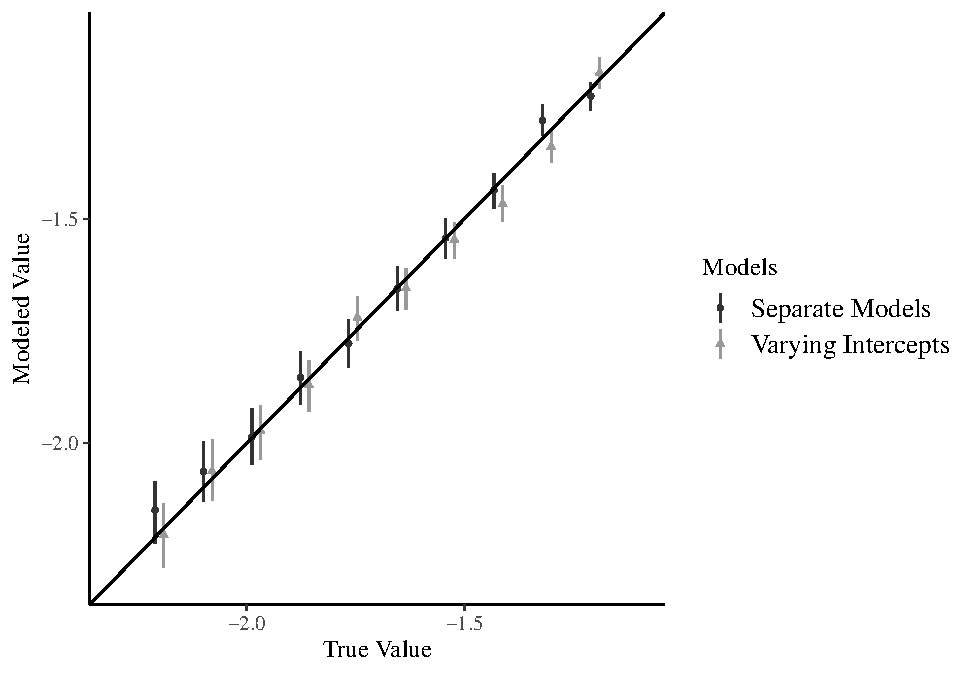
\includegraphics{stan_spectra_manuscript_update_files/figure-latex/unnamed-chunk-3-1.pdf}
\caption{Figure 1. Modeled estimates (median +/- 95\% Credible Intervals
of λ using either 10 separate models or a single model with ten varying
intercepts.\label{single_and_varint_plot:plot}}
\end{figure}

\begin{figure}
\centering
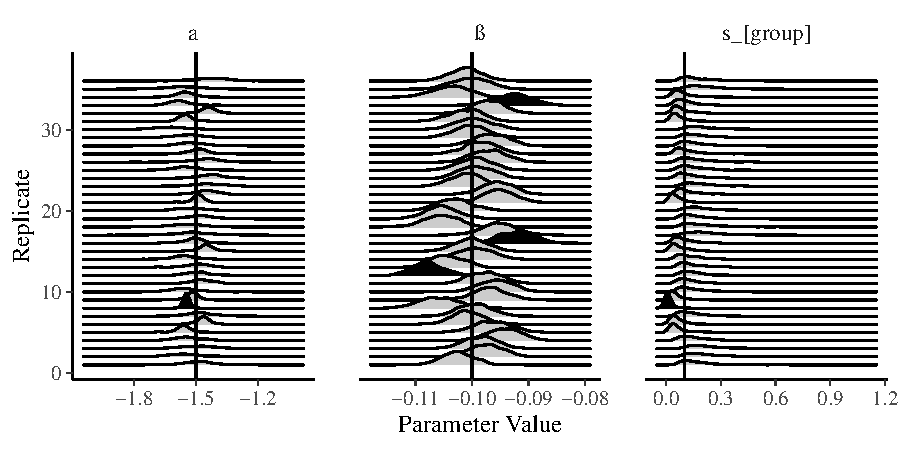
\includegraphics{stan_spectra_manuscript_update_files/figure-latex/unnamed-chunk-4-1.pdf}
\caption{Figure 2. Posterior distributions of n = 20 modeled estimates
of alpha, beta, and sigma\_group for a linear regression estimating the
size spectrum exponent as a function of a continuous predictor. All data
were simulated. Gray densities indicate that the 95\% CrI contains the
true value, while black densities indicate the true values fall outside
of the CrI. The vertical lines indicate true
values.\label{plot_linear_model_bias :plot}}
\end{figure}

\begin{figure}
\centering
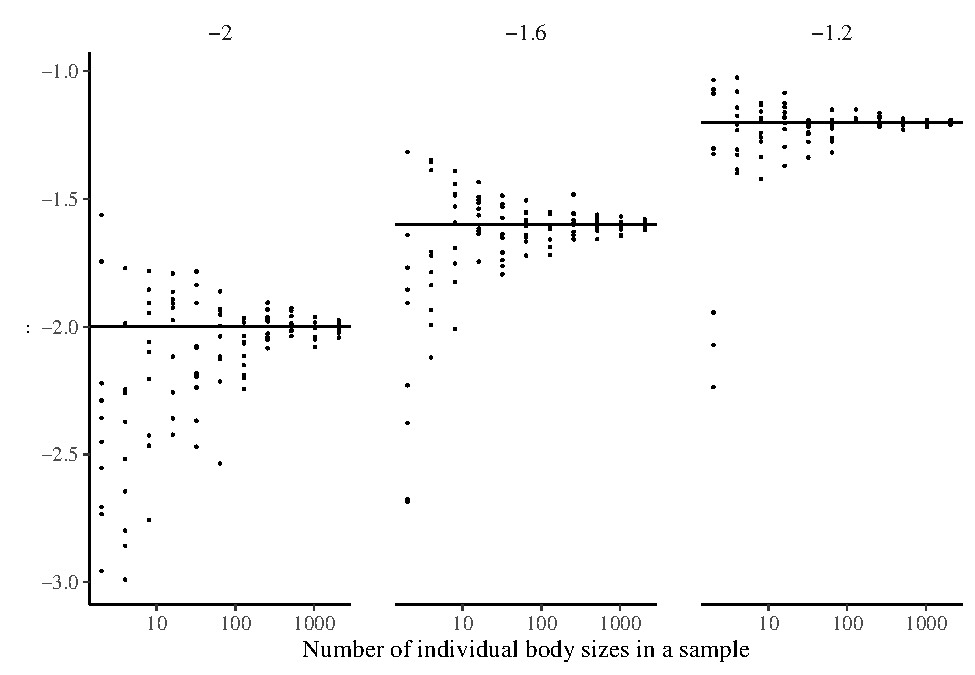
\includegraphics{stan_spectra_manuscript_update_files/figure-latex/unnamed-chunk-5-1.pdf}
\caption{Figure 3. Estimates of λ across 11 different sample sizes
(ranging from 2 to 2048 individuals) and three different true λ's (-2,
-1.6, -1.2). Ten separate models were fit for each of the 11 sample
sizes. The horizontal lines show the true value of λ}
\end{figure}

\begin{figure}
\centering
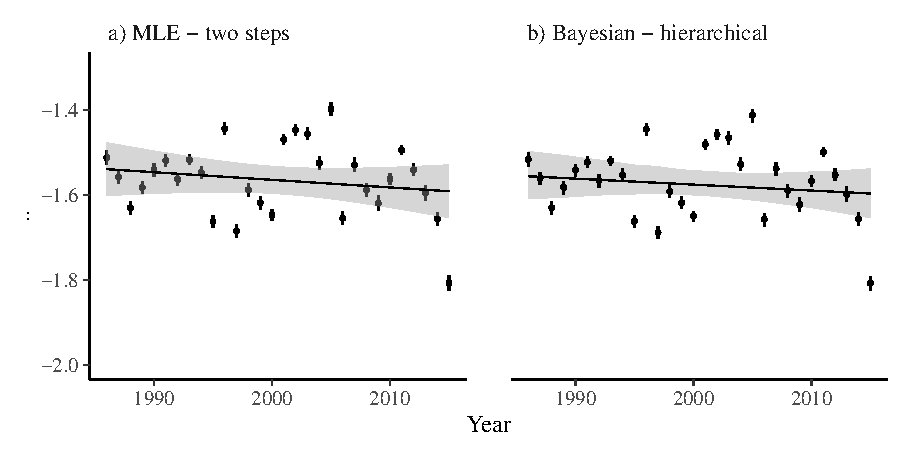
\includegraphics{stan_spectra_manuscript_update_files/figure-latex/unnamed-chunk-6-1.pdf}
\caption{Figure 4. Regression results from a) Edwards et al.~(2020)
using maximum likelihood and linear regression (two steps), b) the
Bayesian model with a paretocounts lpdf (one step), but without varying
intercepts, and c) the Bayesian model with varying intercepts. In a) the
points represent maximum likelihood estimates calculated separately for
each year. In c) they represent hierarchical varying intercepts
calculated from the model. There are no points in (b) because the model
does not estimate lambda for individual years.}
\end{figure}

\hypertarget{section}{%
\section{}\label{section}}

\end{document}
